\chapter{Elastic Scatter of $^8$B Solar Neutrinos in SNO+}
\label{ch:es}

During the water phase of SNO+, after the upgrades made to the SNO detector were commissioned, the detector operated stably for a period of time, producing a physics dataset.
Because of its depth, SNO+ has much lower cosmic muon flux than other water Cherenkov detectors, so even though it is much smaller than, for instance, Super Kamiokande, it is able to make competitive measurements because of lower cosmogenic backgrounds.
These very low backgrounds also enable measurements of solar neutrinos down to low energy thresholds.
The analysis described here does just that by performing a measurement of the $^8$B solar neutrino flux using the elastic scatter (ES) interaction channel.
This also represents the first physics results from the SNO+ detector, and also serves as a cross check that SNO+ is correctly simulating its direction resolution.

\section{Introduction}
\label{sec:solar:intro}

SNO+'s water phase differs from SNO in that light water is used instead of heavy water.
This means that there is no CC or NC interaction, however, there are still electrons present, so the ES process is unchanged.
As described in earlier chapters, the final state electron in the ES interaction has a direction highly correlated with the incident neutrino direction, and this fact can be used to statistically identify ES events in the detector.
This can be achieved by binning events in the observable $\cos{\theta_{sun}}$ which is the cosine of the angle between reconstructed event direction and the Sun at the time of the event.
A maximum likelihood fit as described in \Cref{fit_impl}, but using this reduced observable space, can then be performed to extract the observed flux.

\subsection{Solar ES Signal}
\label{sec:solar:inputs}

As with other maximum likelihood fits, PDFs for the solar events must be generated.
SNOMAN from SNO is replaced by RAT for SNO+, however, both operate very similarly: types of interactions can be simulated and reconstructed like data to build PDFs for statistical analysis of detector data.
Both $\nu_e$ and $\nu_a$ ($\nu_\mu$ and $\nu_\tau$) events are generated with a known flux and flat ($100\%$) survival/transition probability.
This is done for the same reason as in SNO analyses: the neutrino oscillation model is applied as part of the analysis by reweighting events.
The code from the neutrino lifetime analysis presented earlier was leveraged here to produce survival probabilities shown in \Cref{fig:solar:msw} corresponding to the most up-to-date neutrino parameters available from the Particle Data Group \cite{pdg}.

\begin{figure}
\centering
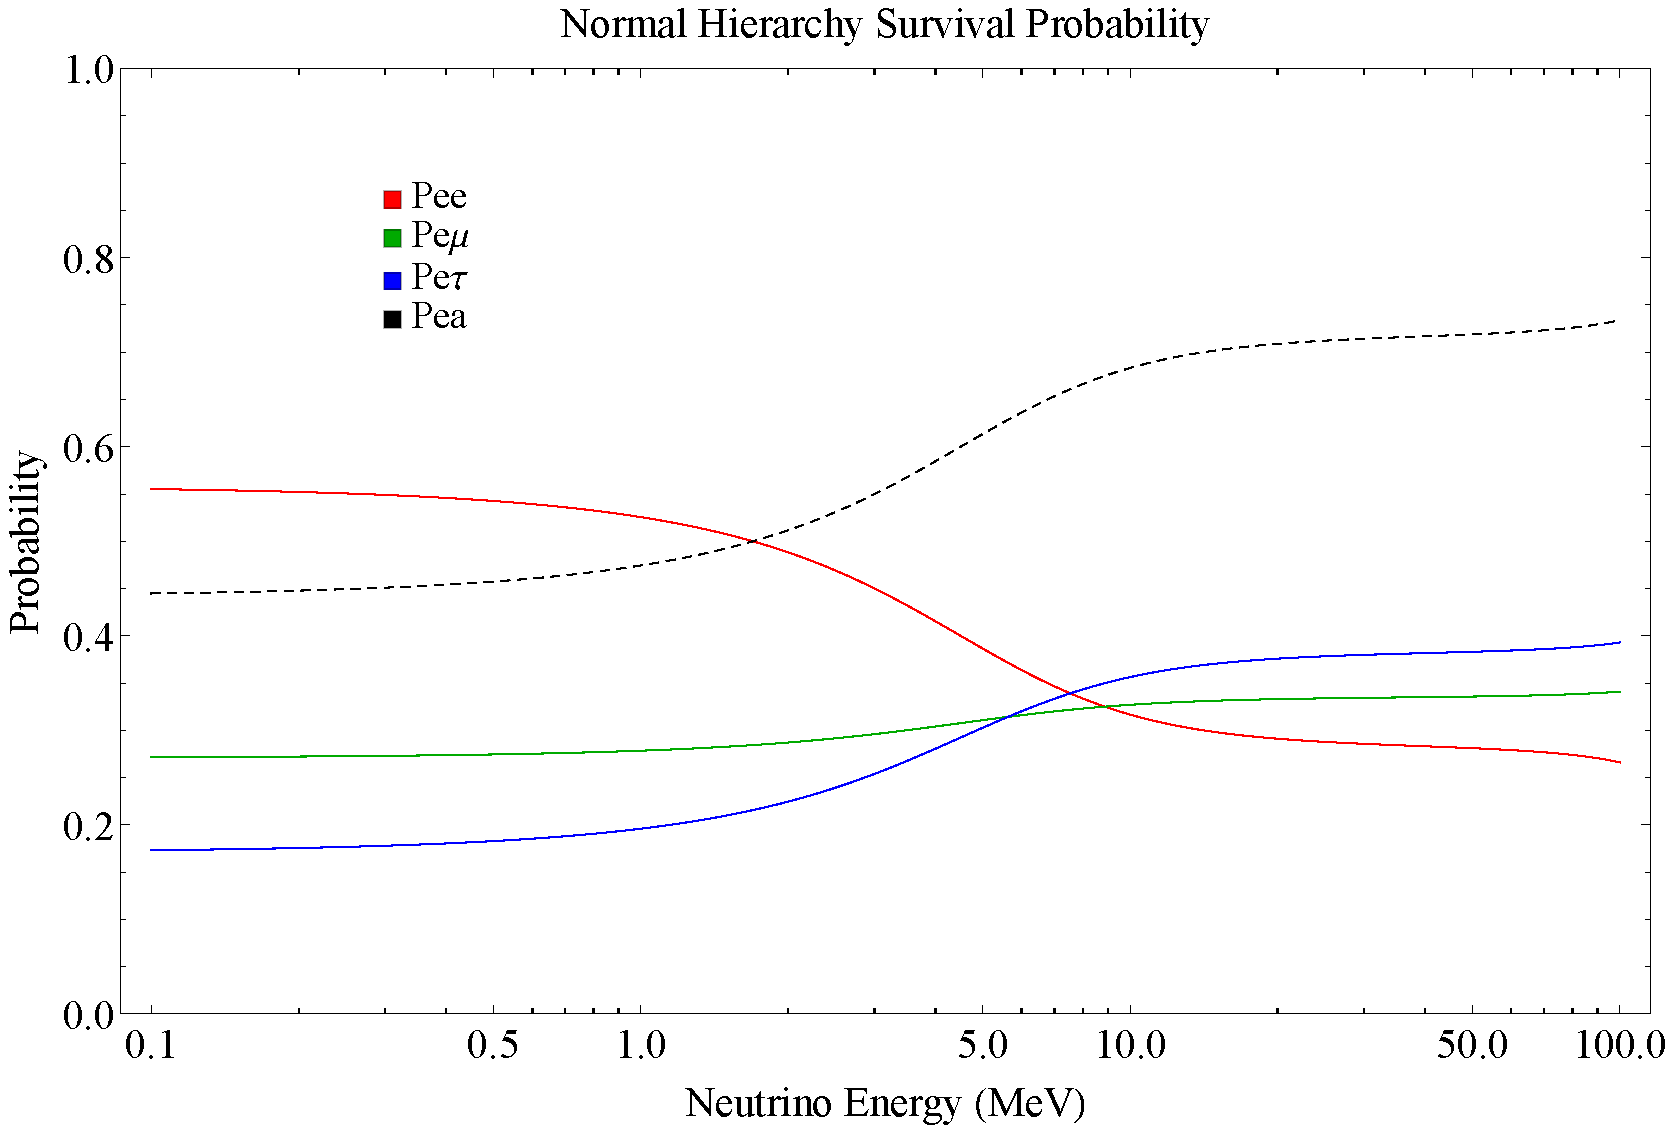
\includegraphics[width=0.8\textwidth]{normal_survival_b8density}
\caption{The MSW survival probability curves used in the SNO+ ES analysis.}
\label{fig:solar:msw}
\end{figure}

Each simulated event is weighed by either $P_{ee}$ for $\nu_e$ or $P_{ea}$ for $\nu_a$ as they are added to a PDF to incorporate known effects of neutrino oscillation.
The relative weights of $\nu_e$ and $\nu_a$ in the PDF is determined by the ES cross section.
RAT MC was generated with the $^8$B flux from BS05(OP) \cite{bs05op}, but this was rescaled to a more up-to-date measured value \cite{GlobalSolarFlux}.
Example PDFs can be seen in \Cref{fig:solar:pdfs}.

\begin{figure}
\centering
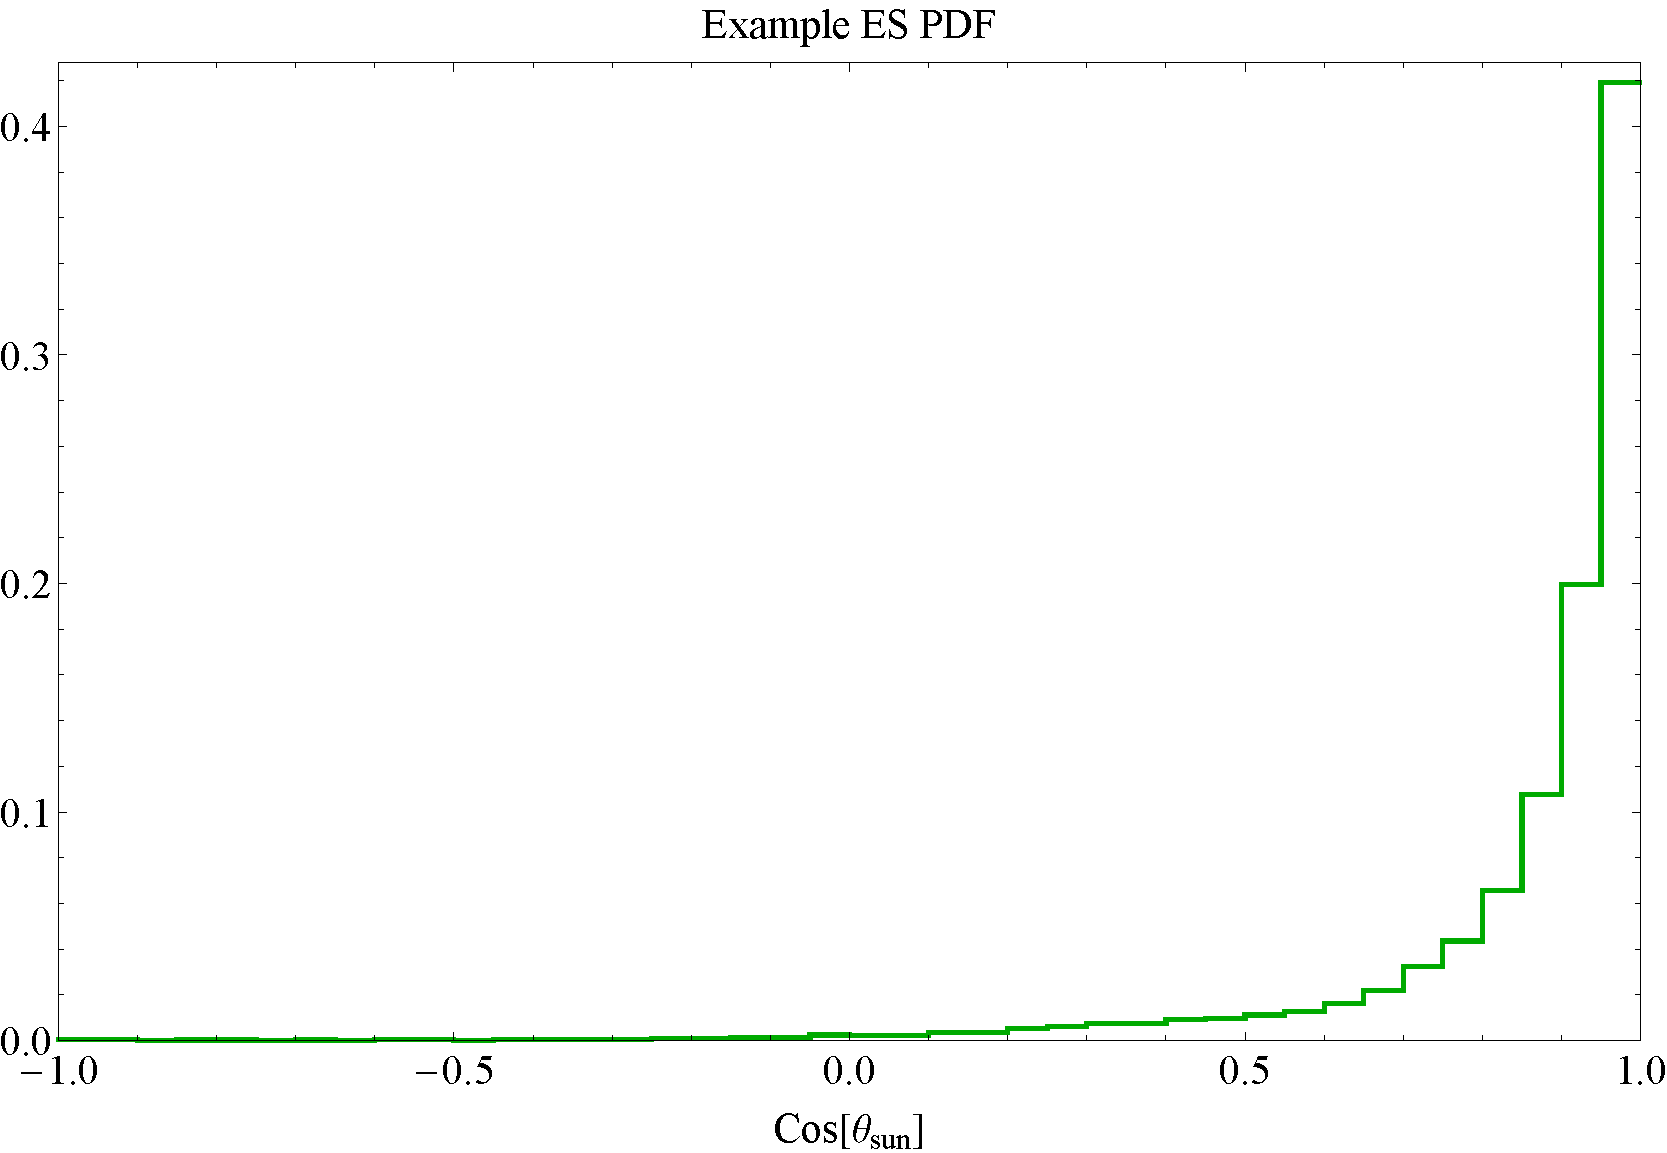
\includegraphics[width=0.8\textwidth]{example_pdf}
\caption{Example PDF for the ES interaction in SNO+.}
\label{fig:solar:pdfs}
\end{figure}

\subsection{Backgrounds}

Since this analysis is only using the observable $\cos{\theta_{sun}}$, the handling of backgrounds is quite simple.
In short, no other types of event are expected to be correlated with the direction of the Sun, so a flat PDF can be used.
This is demonstrated by generating background PDFs as shown in Figure \ref{fig:solar:backgrounds} of all backgrounds considered for SNO+.
Notably, all backgrounds are flat in $\cos{\theta_{sun}}$ as expected.
Using MC derived PDFs offers no benefit here, so an analytically flat PDF is assumed.

\begin{figure}
\centering
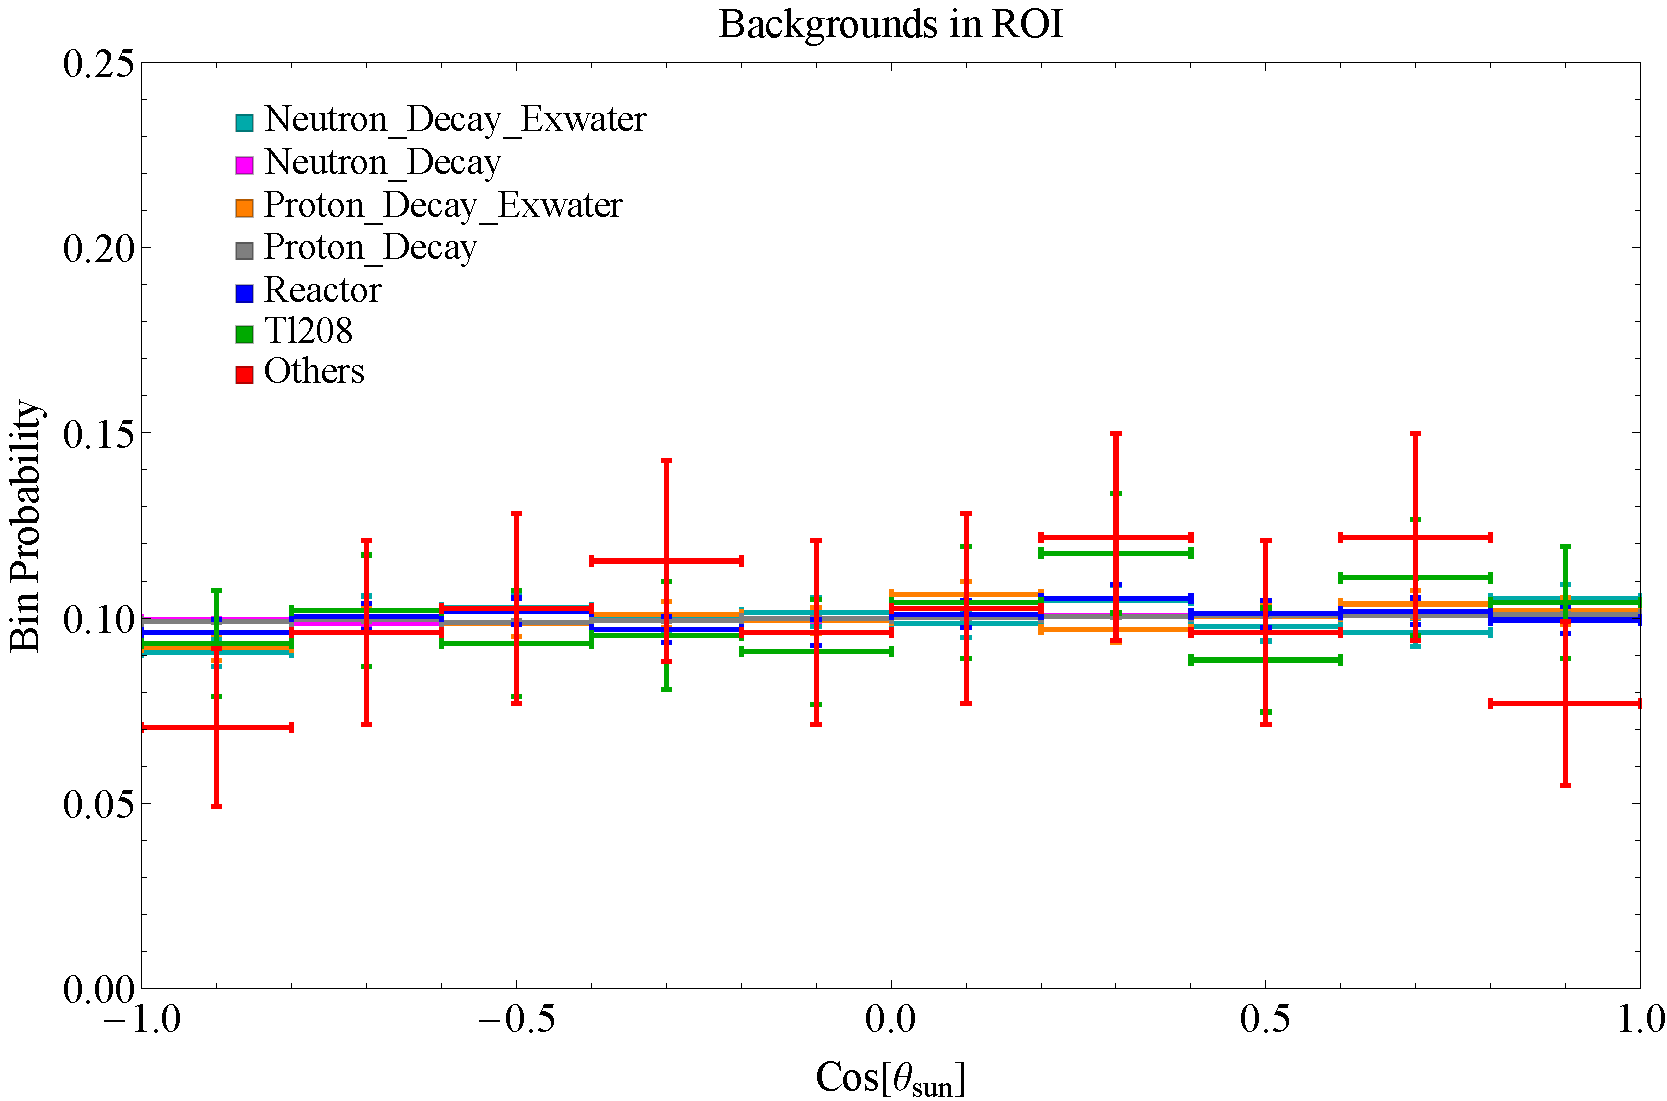
\includegraphics[width=0.8\textwidth]{backgrounds_roi}
\caption{Backgrounds shown binned in the observable $\cos{\theta_{sun}}$ after solar analysis cuts are applied.
Note that backgrounds with fewer than 100 counts were combined and shown as as other.}
\label{fig:solar:backgrounds}
\end{figure}

\section{Data Selection}

As this is an early look at SNO+ data, the criteria defining which events are physics and should be analyzed are not as well defined as they are for contemporary analyses of SNO data.
This section discusses these criteria in detail, and aims to produce a set of data free of instrumental backgrounds by defining low level cuts on detector behavior and basic event information, and high level cuts on reconstructed quantities.

For SNO+ the data within the water phase were separated into various time bins roughly correlated to the background levels during data taking.
This is of interest because different cuts were used for these different timebins.
These data selection criteria described in the following sections were also applied in the process of building PDFs to MC simulation for each time bin to correctly account for the varrying acceptance these different cuts imply.

\subsection{Low Level Cuts}

The SNO+ trigger system records a 32 bit integer where each bit is a boolean mask of the state of the trigger system for each event.
This trigger word identifies, at a very low level, what caused the detector to take data.
Low level event selection requires that the trigger word include a physics trigger based on the number of coincidentally hit PMTs, and excludes any externally forced triggers that may be in the data.
The following expression evaluates to logical false for selected events.

\begin{verbatim}
!(trig_word & 0x3F) || (trig_word & 0xBEF9400)
\end{verbatim}

Various data cleaning classifiers are run over the raw data as part of reconstruction, with the goal of identifying instrumental backgrounds or other non-physics events.
These classifiers produce another 32 bit word which can be checked for event quality.
A check of the data cleaning word requires that all standard data cleaning classifiers did not mark the event as dirty using the analysis mask 0x7FFE.
The following expression evaluates to logical false for selected events.

\begin{verbatim}
((dc_applied & ANALYSIS_MASK) & dc_flagged ) != (dc_applied & ANALYSIS_MASK)
\end{verbatim}

\subsection{High Level Cuts}

Once an event satisfies low level even selection criteria, the results of event reconstruction can be considered.
A valid reconstruction result is then required, meaning the reconstruction algorithms successfully converged to some value.
High level cuts are applied on the in time ratio (ITR), representing the number of hit PMTs within a prompt time window to all hit PMTs, and isotropy ($\beta_{14}$), representing the isotropy of the pattern of hit PMTs.
The region of interest (ROI) for the analysis is then selected with cuts on energy and radius.
Note that initially this analysis only planned to extend down to 5.5 MeV, however evaluation of the actual data indicated that backgrounds were low enough to consider events down to 4.5 MeV.
Other analyses of this data identified a region of high radioactivity near the top of the detector, and for this a z dependent radial cut was adopted.
These high level cuts are summarized per time bin in Table \ref{tbl:solar:roi}.

\begin{table}[]
\begin{center}
\begin{tabular}{l|c|c|c}
\textbf{Time Bin} & Open & External Hotspot & Steady State  \\ \hline
\textbf{Run Range} & 100000-100399 & 100400-102048 & 102049-103402 \\ \hline
\textbf{Criteria} & ITR $ \geq 0.55$ & ITR $ \geq 0.55$ & ITR $ \geq 0.55$ \\
& $-0.12 \leq \beta_{14} \leq 0.95$ & $-0.12 \leq \beta_{14} \leq 0.95$ & $-0.12 \leq \beta_{14} \leq 0.95$ \\
& $4.5 \leq E \leq 15.0$ & $4.5 \leq E \leq 15.0$ & $4.5 \leq E \leq 15.0$ \\
& $R \leq 5.3$ & $R \leq 5.3$ (for Z$<$0) & $R \leq 5.3$ \\
& & $R \leq 4.2$ (for Z$>$0) & \\
\end{tabular}
\\[2\baselineskip]
\begin{tabular}{l|c|c|c}
\textbf{Time Bin} & AV 1 \& 2 & AV 3 \& 4 & Post-Bubble \\ \hline
\textbf{Run Range} & 103411-105171 & 105493-105661 & 106716- \\
& & 106070-106499 & \\ \hline
\textbf{Criteria} & ITR$ \geq 0.55$ & ITR$ \geq 0.55$ & ITR$ \geq 0.55$ \\
& $-0.12 \leq \beta_{14} \leq 0.95$ & $-0.12 \leq \beta_{14} \leq 0.95$ & $-0.12 \leq \beta_{14} \leq 0.95$ \\
& $4.5 \leq E \leq 15.0$ & $4.5 \leq E \leq 15.0$ & $4.5 \leq E \leq 15.0$ \\
& $R \leq 5.3$ & $R \leq 5.3$ & $R \leq 5.3$ \\
\end{tabular}
\caption{The high level cuts used in the SNO+ ES analysis. Selected events will pass these cuts.}
\label{tbl:solar:roi}
\end{center}
\end{table}

\section{Systematic Uncertanties}

With the procedure described above for generating signal and background PDFs, the extended maximum likelihood fit is straightforward.
The remaining concern are systematic uncertainties that might be present between the data and simulated events.
For this analysis, systematics are primarily propagated primarily by varying a systematic uncertainty parameter, rerunning the analysis, and recording the variation in the results.
As a final step, the variations from all systematics are combined in quadrature to arrive at the total systematic uncertainty.
This assumes that systematic uncertainties are uncorrelated and their effects normally distributed.

\subsection{Energy Scale and Resolution}

The energy scale and resolution were determined by comparing data from a deployment of the \N calibration source to MC. 
This yielded a $2.9\%$ uncertainty on the energy scale, and required an additional $10.2\%$ smearing at $5$MeV to be applied to MC to match the data.
To find the smearing at other energies $E$ in MeV, the following equation was assumed
\begin{equation}
\label{eqn:solar:esmear}
E_{smear} = 0.102\sqrt{5 E}.
\end{equation}

To propagate the energy scale systematic, the MC reconstructed energy was scaled up and down by $2.9\%$ and the analysis performed again with each condition.
The resulting variation in the fitted measured flux was taken as the systematic uncertainty on the flux.
The energy resolution systematic was propagated by smearing the reconstructed MC energies by \ref{eqn:solar:esmear} and then rerunning the fit.
Again, the resulting variation in the measured flux is taken as the systematic uncertainty.

\subsubsection{Reconstructed Energy Correction}

Comparison of the \N calibration data to MC demonstrated that the energy reconstruction algorithm was not performing optimally.
From this calibration data an energy correction lookup table applied to both data and MC was derived.
Further analysis of \N calibration data demonstrated radius- and z-dependent energy scale bias in the energy reconstruction algorithm that was corrected by applying the following scaling to the reconstructed energy
\begin{equation}
1 + A + ( (1 + B \rho^2)(1 + Cz + Dz^2 + Ez^3) - 1 )
\end{equation}
where $A$, $B$, $C$, $D$, and $E$ were determined separately for data and MC.

\subsection{Position Scale and Resolution}

As the solar MC is simulated as a uniform distribution inside the AV, and the position resolution of SNO small (O(10cm)), smearing the reconstructed position by this resolution has a 
negligible effect on the expected number of events.
However, this uncertainty is propagated similar to the energy resolution systematic: by smearing the MC reconstructed positions by the position resolution and rerunning the analysis.
The more important position systematic is the position scale, as this changes the fiducial volume which is directly proportional to the measured flux.
The vertex scale systematic is determined for each axis by comparing \N data to MC, and found uncertainties of $(^{+0.03}_{-0.19}\%,^{+0.03}_{-0.38}\%,^{+0.03}_{-0.37}\%)$.
To propagate these systematics the axes were simultaneously scaled up and down by these values, and the fit was rerun.

\subsection{Angular Resolution}

Previously the uncertainty in angular resolution was accounted for by remapping the $\cos{\theta_{sun}}$ observable using the equation
\begin{equation}
\cos{\theta'_{sun}} = 1 + \frac{\cos{\theta_{sun}}-1}{1\pm\Delta}
\label{solar:eq:dirres}
\end{equation}
where $\Delta$ is a parameter representing the systematic uncertainty on the angular resolution.
For the solar ES analysis this approach would likely work, however it was noted that this results in events being pushed into non-physical values ($\cos \theta_{sun} < -1$) or leaving a void of zero probability near $\cos \theta_{sun} = 1$.
To handle this better, it was proposed to instead adjust the reconstructed direction of each MC event to be further or nearer the MC truth direction (as determined by  \ref{solar:eq:dirres}), and finally recomputing the $\cos \theta_{sun}$ PDF using these new directions and rerunning the fit.
This method was adopted for the early stages of this analysis.

As the angular systematic was determined to be the dominate systematic, and the solar data well constrains the angular resolution, this final form of this analysis opted to float this uncertainty using the uncertainty determined from an analysis of \N calibration data as a constraint.
This requires re-smearing each event's direction and rebuilding the angular PDF at each step of the fit which is computationally challenging but tractable for this analysis with so few floated variables.

Like the other systematics, the angular resolution was determined by comparing \N data to MC. 
This systematic does strongly affect the shape of the ES PDF as described by Equation \ref{solar:eq:dirres}, and the constraint on $\Delta$ was determined to be $0^{+0.08}_{-0.19}$.

\section{Open Data Analysis}
\label{sec:solar:opendata}

To understand detector data, constrain backgrounds, and aid in the development of analyses, SNO+ provided about 16 days of detector livetime with no blinding applied.
The remaining data was withheld until analyses were developed so that unbiased results could be extracted.

\begin{table}
\centering
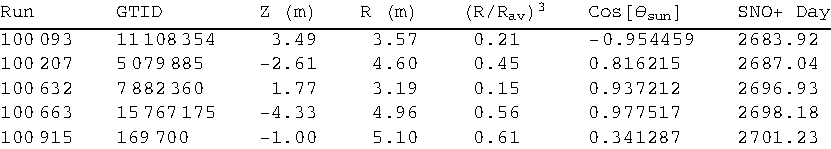
\includegraphics[width=\textwidth]{events}
\caption{The events selected by solar analysis cuts in the open dataset.}
\label{tbl:solar:openev}
\end{table}

The following preliminary diagnostic plots are created with a higher energy threshold of 5.5 MeV.
After applying the data selection criteria to this open data, there are 5 candidate ES events selected.
These candidates are shown with with various observables in Table \ref{tbl:solar:openev}.
The SNO+ date for the runs included along with the 5 selected events is shown in Figure \ref{fig:solar:opendata} to gain confidence that these events are not suspiciously distributed in time.
In a similar vein, the time of day of each event along with the relative livetime (represented by number of runs at that time) is shown in Figure \ref{fig:solar:tod}.

\begin{figure}
\centering
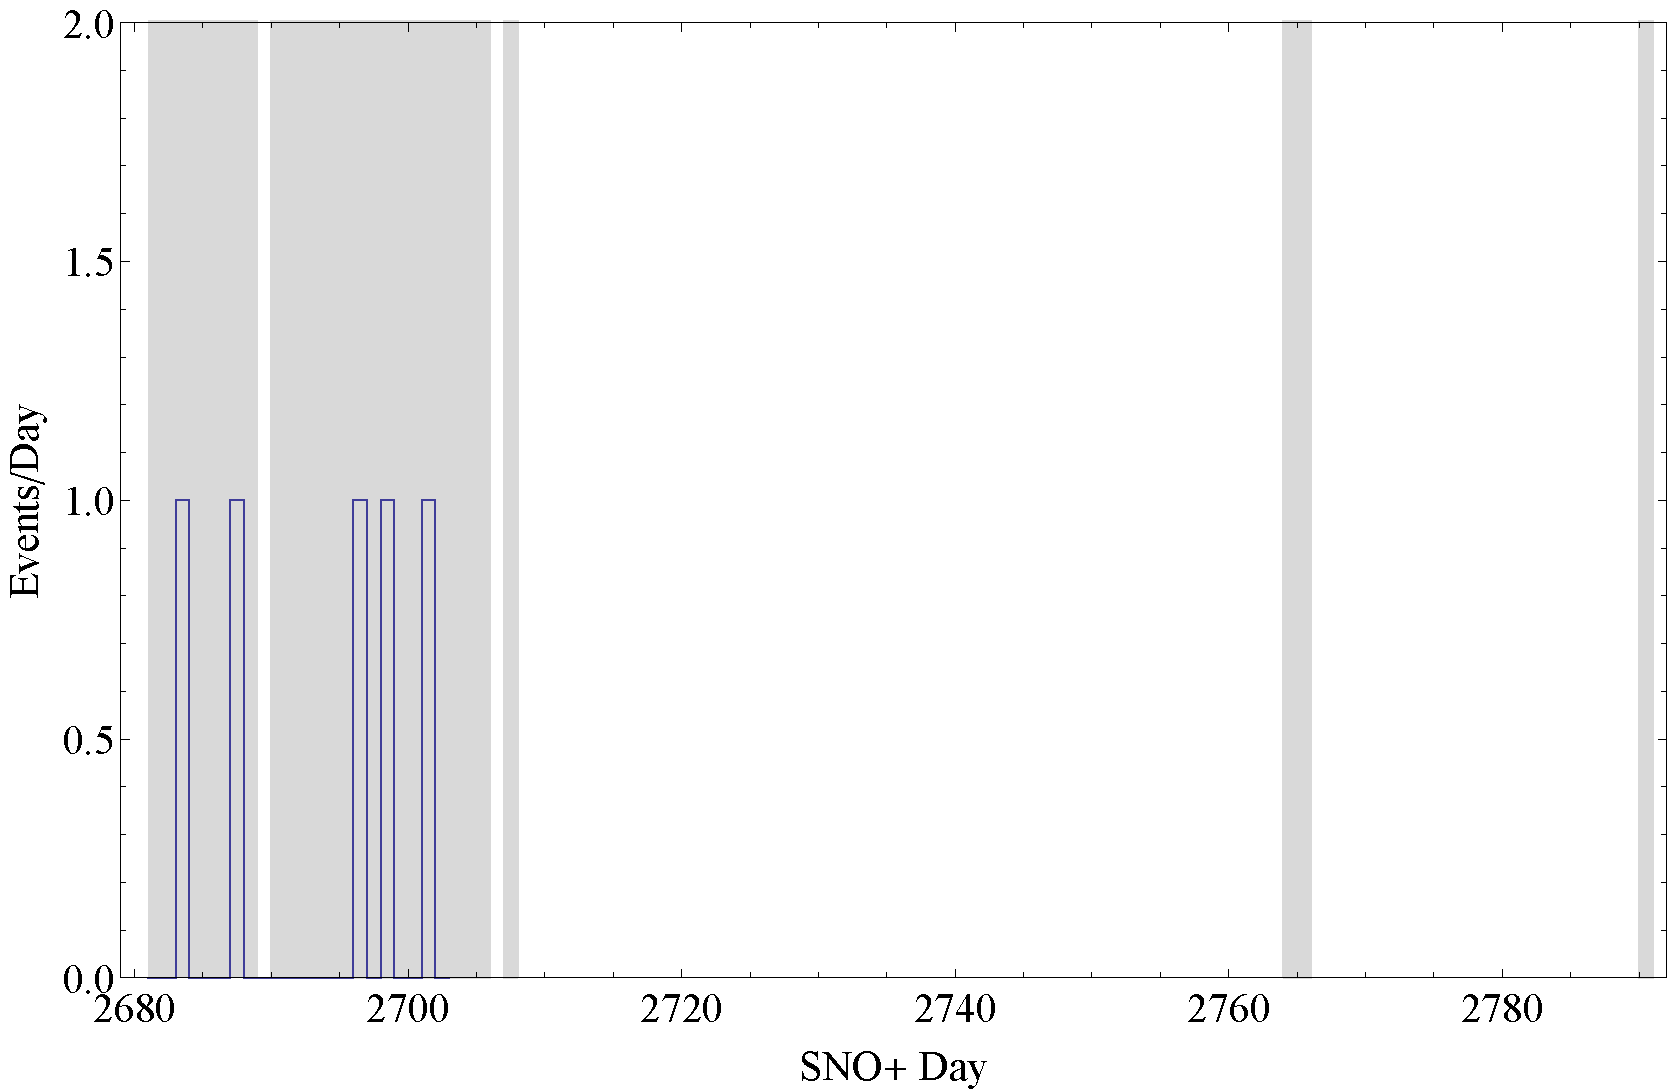
\includegraphics[width=0.8\textwidth]{per_day}
\caption{The SNO+ days that are included in the open data analysis are shown
         shaded gray.
         The date of each selected event in the open data analysis is also shown.}
\label{fig:solar:opendata}
\end{figure}


\begin{figure}
\centering
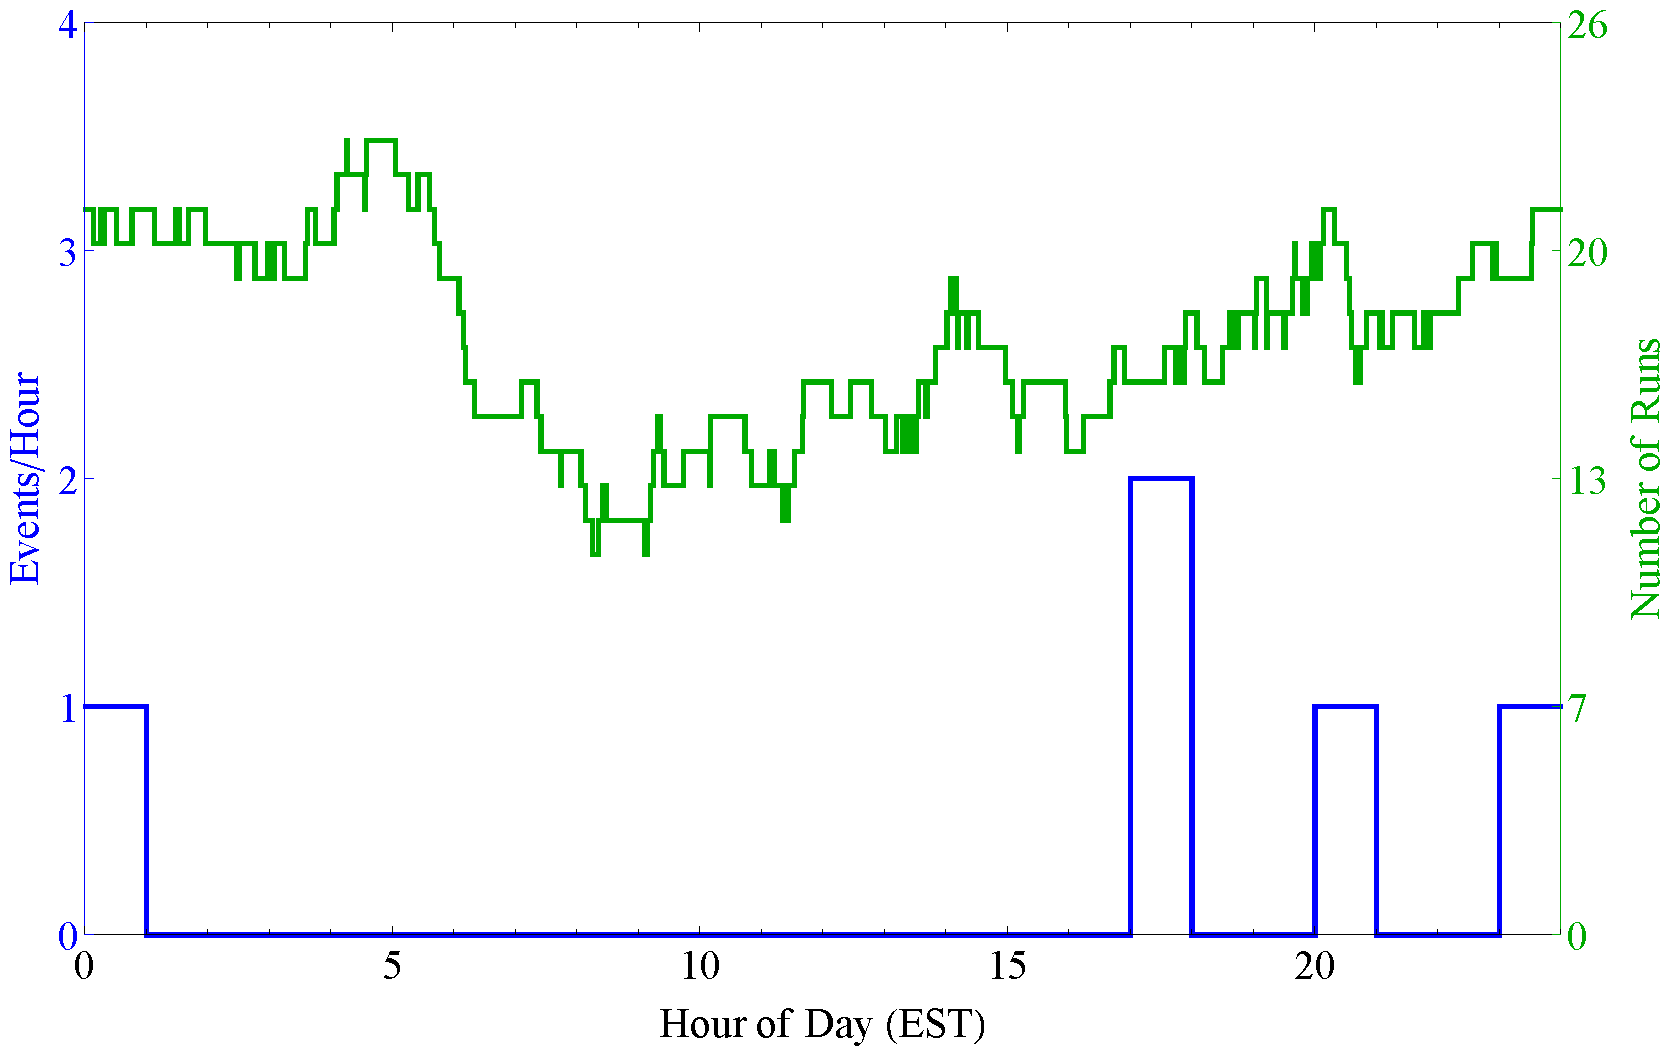
\includegraphics[width=0.8\textwidth]{hour_of_day}
\caption{The time of day (Sudbury timezone, no DST correction) of each selected
         event in the open data analysis.
         Also shown are the number of runs at any particular time of day.}
\label{fig:solar:tod}
\end{figure}


Due to there being so few events in this dataset, a very coarse binning of $0.2$ $\cos{\theta_{sun}}$ intervals is used.
For the open dataset with a 5.5-MeV threshold, a flux scale, the fraction of the expected $^8$B flux, of $0.54\pm0.37$ (stat.) $^{+0.09}_{-0.05}$ (syst.) is found.
The best fit is shown plotted with the binned data in Figure \Cref{fig:solar:open45}.
While this result disagrees with the expected $^8$B flux at over one sigma, it is expected that this is a statistical fluctuation due to very few statistics.

Within SNO+ there is interest in opening up the energy ROI for this analysis to include as many solar events as possible.
To that end, an identical analysis was performed, but with a lower bound on the energy of 4.5 MeV.
This larger energy ROI yields the results \Cref{fig:solar:open55}, which notably agrees better with the expected $^8$B flux and shows higher background expected at lower energies.
The justification for the 4.5 MeV threshold used for all other results in this chapter is the clear ES peak observed in this open data with a 4.5 MeV threshold.

\begin{figure}
\centering
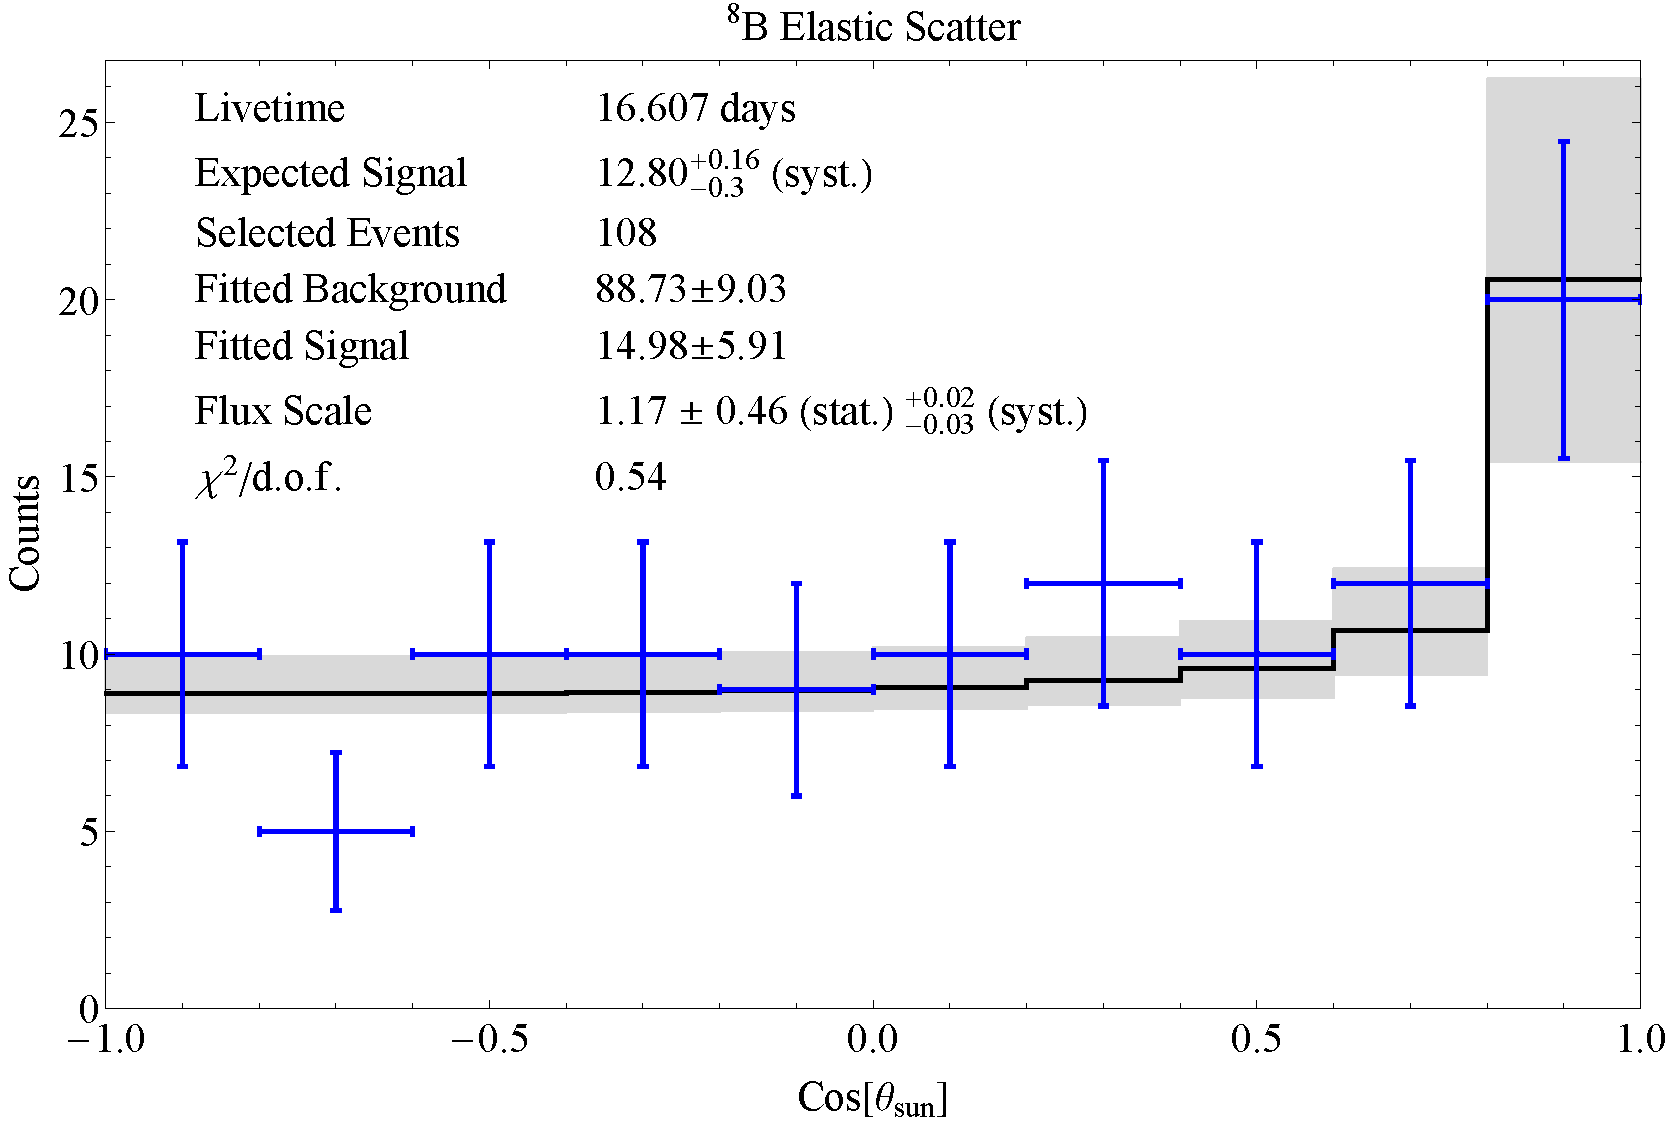
\includegraphics[width=\textwidth]{b8_es_fit_4_5}
\caption{
Summary plot of the $^8$B ES fit on the open dataset using the alternative energy range 4.5-15.0 MeV.
The shaded regions show the fit uncertainty, with the selected events shown in blue.
The fitted flux scale is shown relative to the current global predictions \cite{GlobalSolarFlux}.
}
\label{fig:solar:open45}
\end{figure}

\begin{figure}
\centering
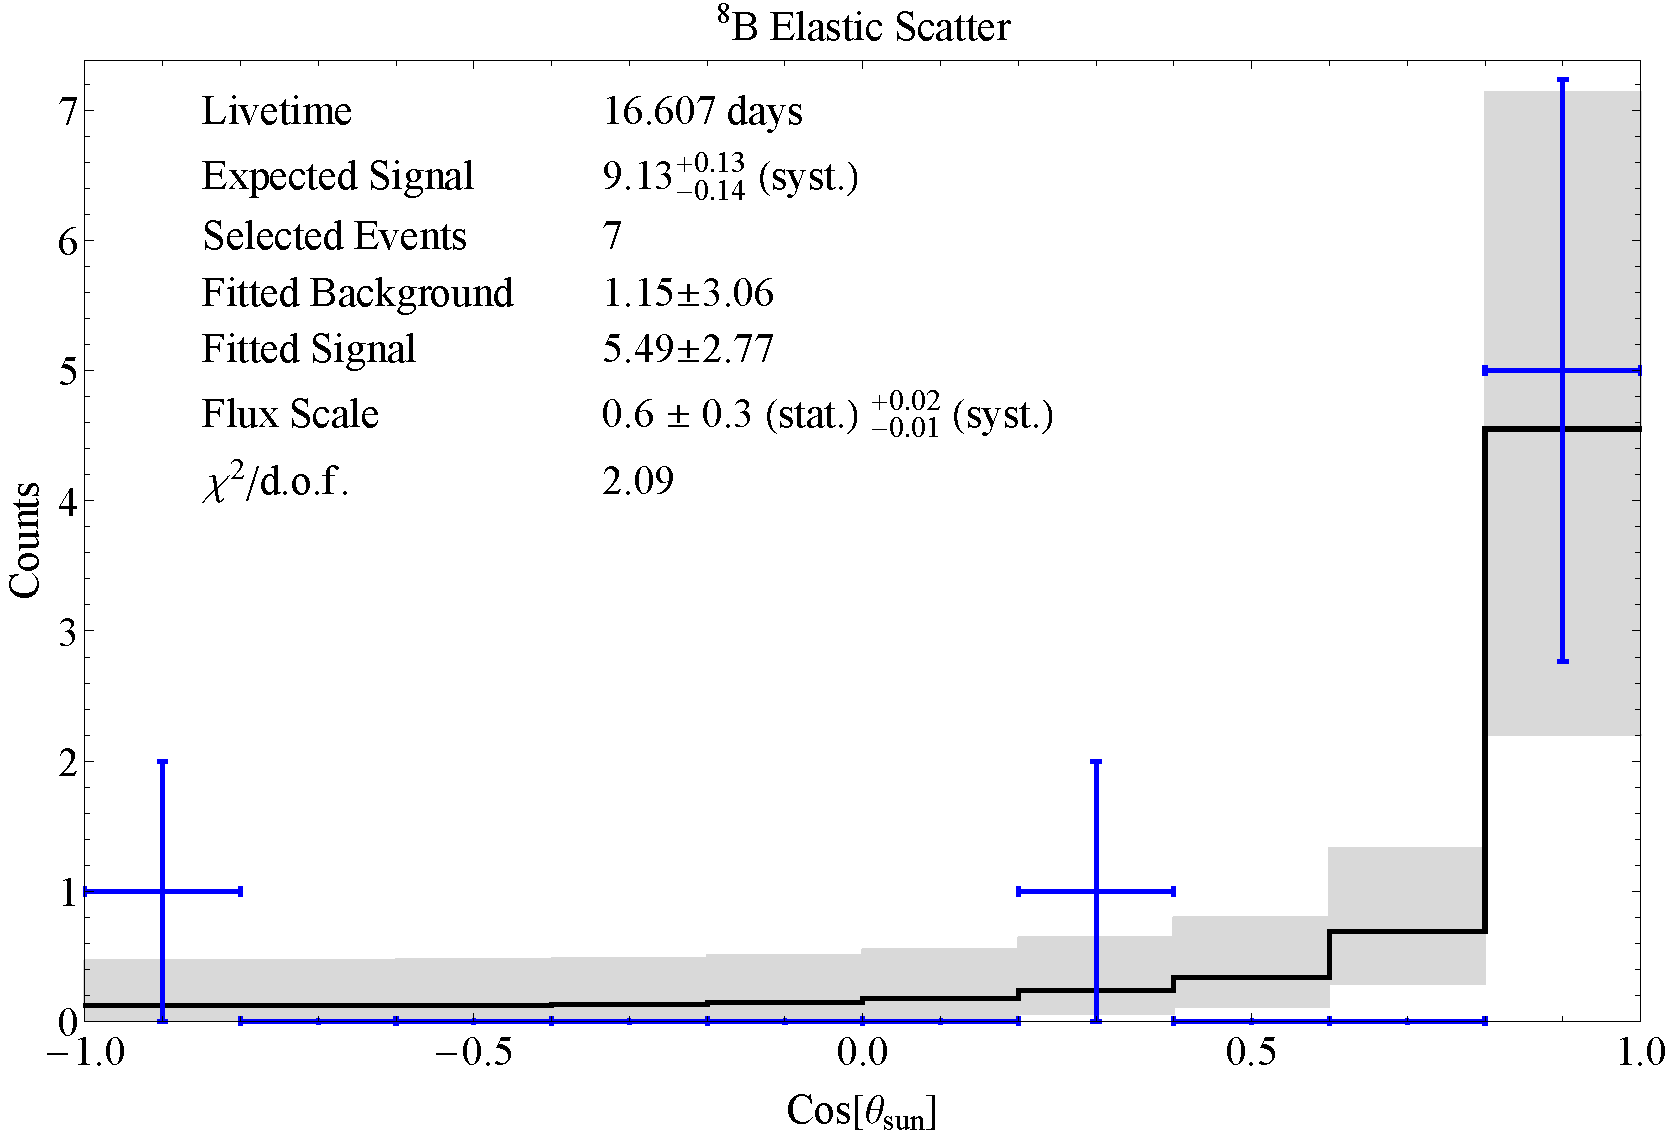
\includegraphics[width=\textwidth]{b8_es_fit_5_5}
\caption{
Summary plot of the $^8$B ES fit on the open dataset using the alternative energy range 5.5-15.0 MeV.
The shaded regions show the fit uncertainty, with the selected events shown in blue.
The fitted flux scale is shown relative to the current global predictions \cite{GlobalSolarFlux}.
}
\label{fig:solar:open55}
\end{figure}

\clearpage

\section{Final Results}
\label{sec:solar:updated}

Following a review of the open data analysis as described in the previous section, the SNO+ Analysis Committee approved the analysis procedure to move ahead with the entire SNO+ water phase dataset.
The additional livetime (approximately 115 days) and additional events this implies allows for finer data binning of 0.05 $\cos{\theta_{sun}}$ intervals.

\begin{figure}
\centering
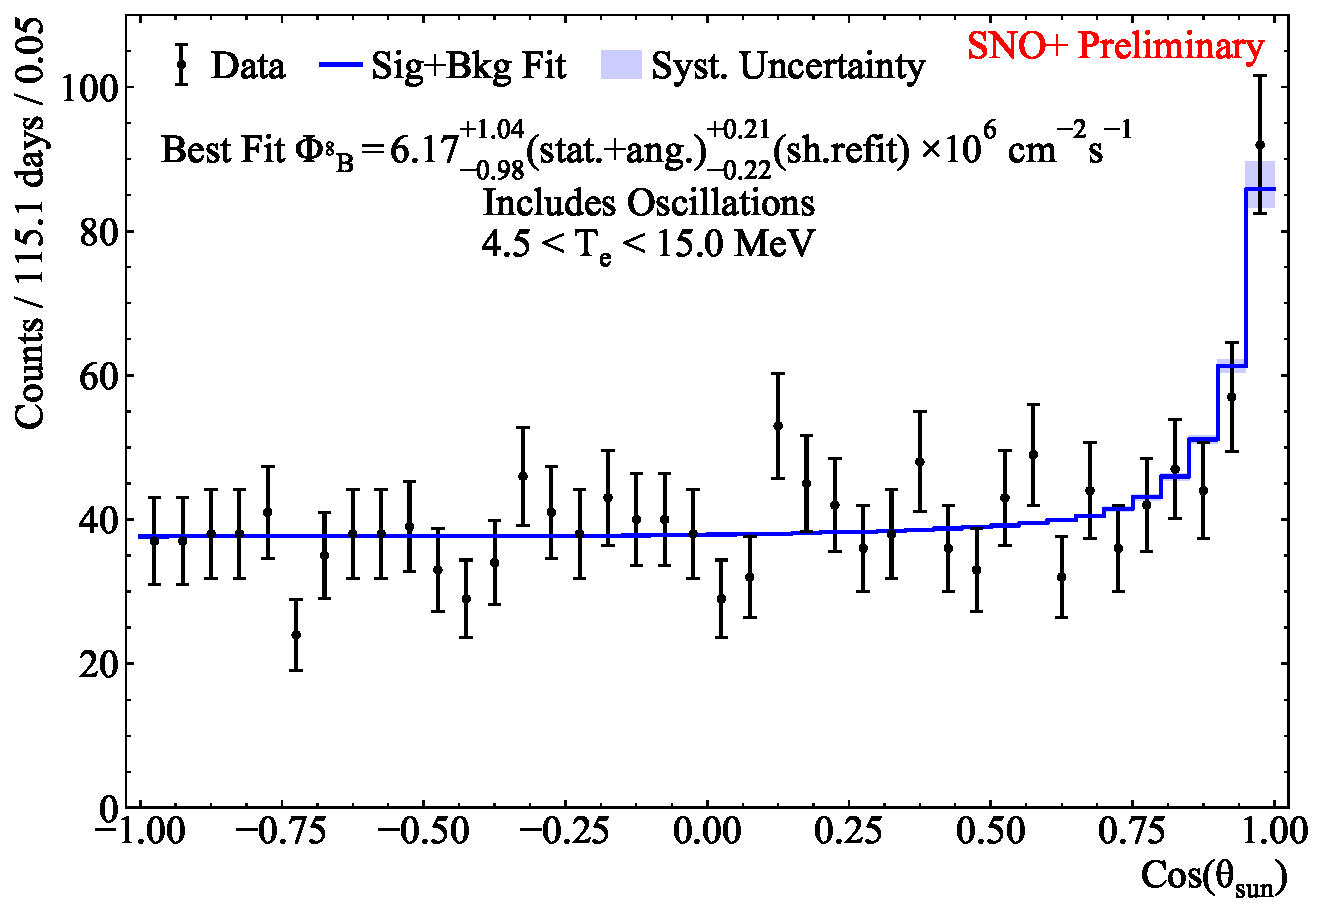
\includegraphics[width=\textwidth]{8b_es_4_5_15_0_fit_float_ang_res}
\caption{Summary plot of the SNO+ $^8$B ES analysis on the full dataset using the energy range $4.5-15.0$ MeV.}
\label{fig:solar:unpdated_fit_4.5}
\end{figure}

\begin{table}[]
\begin{center}
\begin{tabular}{c|c|c|c}
Systematic & Uncertainty & Application & Origin \\ \hline
$E_{scale}$     & $\pm 2.0\%$ & shift-refit $^{+0.0217}_{-0.0204}$ & \N \rule{0pt}{2.6ex}\rule[-1.2ex]{0pt}{0pt}  \\
$E_{res}$       & $\sqrt{(1+0.0018)^2-1.0}\sqrt{E}$ & shift-refit $\pm 0.0005$ & \N  \rule{0pt}{2.6ex}\rule[-1.2ex]{0pt}{0pt}  \\
${XYZ}_{scale}$ & $(^{+0.91}_{-1.01},^{+0.92}_{-1.02},^{+0.91}_{-0.99}) \%$ & shift-refit $^{+0.0261}_{-0.0284}$ & \N  \rule{0pt}{2.6ex}\rule[-1.2ex]{0pt}{0pt}  \\
${XYZ}_{shift}$ & $(^{+16.4}_{-18.2},^{+22.3}_{-19.2},^{+38.4]}_{-16.7})$ mm & shift-refit $^{+0.0002}_{-0.0001}$ & \N  \rule{0pt}{2.6ex}\rule[-1.2ex]{0pt}{0pt}  \\
${XYZ}_{res}$ & $(104.0,98.2,106.2)$ mm & shift-refit $\pm 0.0002$ & \N \rule{0pt}{2.6ex}\rule[-1.2ex]{0pt}{0pt}  \\
Dir$_{res}$     &  $\Delta = ^{+0.08}_{-0.13}$ & floated (best fit $\Delta = -0.02^{+0.09}_{-0.13}$) & \N \rule{0pt}{2.6ex}\rule[-1.2ex]{0pt}{0pt}  \\ \hline
\end{tabular}
\caption{ Systematic uncertainties considered on the SNO+ ES analysis are shown here.
The impact shown for shift-and-refit parameters is a fractional change of the $^8$B flux from the central value of the fit for the energy range $4.5-15.0$ MeV.
For the livetime considered in this analysis approximately 100 solar ES events are expected.}
\label{tbl:solar:updated_syst}
\end{center}
\end{table}

Using the full dataset, the full energy range $4.5-15.0$ MeV can be fit. 
The results of this fit is shown in Figure \ref{fig:solar:unpdated_fit_4.5} and can also be found in \cite{snoplus_solar}.
\Cref{tbl:solar:updated_syst} shows in detail the impact of each systematic uncertainty. 
Notably this fit is consistent with the current global best fit for the $^8$B neutrino flux, $5.16^{+0.13}_{-0.09}$(stat)$^{+0.30}_{-0.26}$(syst) \cite{GlobalSolarFlux}, and demonstrates that SNO+ has achieved very low backgrounds as evidenced by the clear ES peak in the solar direction despite the very low $4.5$ MeV threshold.
